\documentclass[tikz]{standalone}

\usepackage{amsfonts}
\usepackage{amsmath}
\usepackage{braket}

\usepackage{tikz}
\usetikzlibrary{shapes.geometric,patterns,positioning,matrix}
\usetikzlibrary{shadows,calc,3d,arrows.meta,decorations.pathmorphing,decorations.markings,decorations.pathreplacing}

\definecolor{googleB}{HTML}{4285F4}
\definecolor{googleG}{HTML}{34A853}
\definecolor{googleY}{HTML}{FBBC05}
\definecolor{googleR}{HTML}{EA4335}
\definecolor{googleBG}{HTML}{3B96A4}

% load TikZ grafic definitions
%\input{gfx_TikZ}

% main document
\begin{document}

	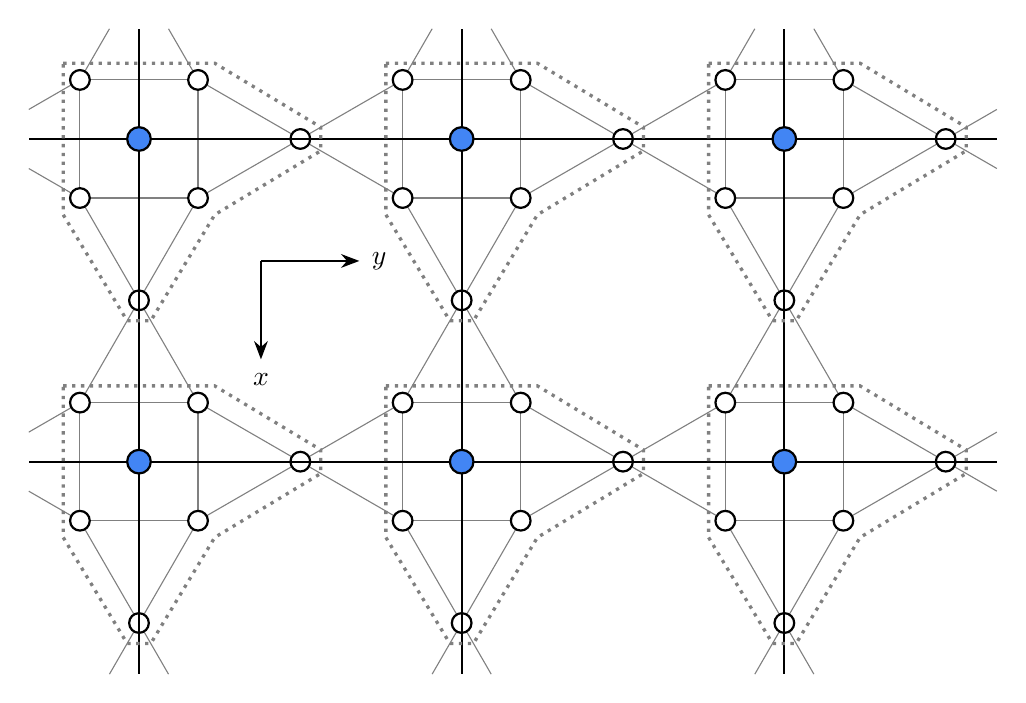
\begin{tikzpicture}

		\def\disL{0.75}
        \def\tensorSizeL{0.125}
		\def\tensorSizeS{0.150}

		\begin{scope}[shift = {(-0.5, +0.5)}]
			\draw[thick, -{Stealth[scale = 1.0]}] (0, 0) to (0, -1.25) node at (0, -1.50) {$x$};
			\draw[thick, -{Stealth[scale = 1.0]}] (0, 0) to (+1.25, 0) node at (+1.50, 0) {$y$};
		\end{scope}

		\foreach \x in {-1, +1, +3} {

			\foreach \y in {-1, +1} {

				\begin{scope}[shift = {({\x * \disL + \x * tan(60) * \disL}, {\y * \disL + \y * tan(60) * \disL})}]

					% define Square-Kagome lattice coordiates
					% \coordinate (1) at ($(0, {-\disL - tan(30) * \disL}) + (270 : {\disL / cos(30)})$);
					\coordinate (1) at (0, {- \disL - \disL / tan(30)});
					\coordinate (2) at (-\disL, -\disL);
					\coordinate (3) at (-\disL, +\disL);
					\coordinate (4) at (+\disL, -\disL);
					\coordinate (5) at (+\disL, +\disL);
					% \coordinate (6) at ($({+\disL + tan(30) * \disL}, 0) + (  0 : {\disL / cos(30)})$);
					\coordinate (6) at ({+\disL + \disL / tan(30)}, 0);

					% define iPESS coordinates
					\coordinate (SL) at ({-\disL - tan(30) * \disL}, 0);
					\coordinate (SU) at (0, {+\disL + tan(30) * \disL});
					\coordinate (SR) at ({+\disL + tan(30) * \disL}, 0);
					\coordinate (SD) at (0, {-\disL - tan(30) * \disL});

					% Square-Kagome lattice links
					\draw[gray] (2) to (3) to (5) to (4) -- cycle;

					\draw[gray] (1) to ($(1) + ( 60 : \disL)$);
					\draw[gray] (1) to ($(1) + (120 : \disL)$);
					\draw[gray] (1) to ($(1) + (240 : \disL)$);
					\draw[gray] (1) to ($(1) + (300 : \disL)$);

					\draw[gray] (2) to ($(2) + (150 : \disL)$);
					\draw[gray] (2) to ($(2) + (300 : \disL)$);

					\draw[gray] (3) to ($(3) + ( 60 : \disL)$);
					\draw[gray] (3) to ($(3) + (210 : \disL)$);

					\draw[gray] (4) to ($(4) + (240 : \disL)$);
					\draw[gray] (4) to ($(4) + ( 30 : \disL)$);

					\draw[gray] (5) to ($(5) + (330 : \disL)$);
					\draw[gray] (5) to ($(5) + (120 : \disL)$);

					\draw[gray] (6) to ($(6) + ( 30 : \disL)$);
					\draw[gray] (6) to ($(6) + (150 : \disL)$);
					\draw[gray] (6) to ($(6) + (210 : \disL)$);
					\draw[gray] (6) to ($(6) + (330 : \disL)$);

					% Square-Kagome lattice sites
					\foreach \site in {1, 2, 3, 4, 5, 6} {
						\draw[thick, fill = white] (\site) circle (\tensorSizeL);
					}

					% draw coarse-grained tensor
					\draw[thick] (0, 0) to ($(-\disL, 0) + 0.5*(150 : {\disL}) + 0.5*(210 : {\disL})$);
					\draw[thick] (0, 0) to ($(0, +\disL) + 0.5*(60 : {\disL}) + 0.5*(120 : {\disL})$);
                    \draw[thick] (0, 0) to ($(0, {- \disL - \disL / tan(30)}) + 0.5*(240 : {\disL}) + 0.5*(300 : {\disL})$);
					\draw[thick] (0, 0) to ($({+ \disL + \disL / tan(30)}, 0) + 0.5*(30 : {\disL}) + 0.5*(330 : {\disL})$);
                    \draw[thick, fill = googleB] (0, 0) circle (\tensorSizeS);


					% draw unit cell borders
					\draw[gray, very thick, dotted] ($(3) + (135 : 0.30)$) to ($(5) + ( 45 : 0.30)$) to ($(6) + ( 30 : 0.30)$) to ($(6) + (330 : 0.30)$) to ($(4) + (315 : 0.30)$) to ($(1) + (300 : 0.30)$) to ($(1) + (240 : 0.30)$) to ($(2) + (225 : 0.30)$) -- cycle;

				\end{scope}
			}

		}

	\end{tikzpicture}

\end{document}

%%% Local Variables:
%%% mode: latex
%%% TeX-master: t
%%% End:
